\documentclass[
  11pt,
  letterpaper,
   addpoints,
   answers
  ]{exam}

\usepackage{../exercise-preamble}

\begin{document}

\noindent
\begin{minipage}{0.47\textwidth}

\includegraphics[width=\textwidth]{../fcfm_die}
\end{minipage}
\begin{minipage}{0.53\textwidth}
\begin{center} 
\large\textbf{Conversión de la Energía y Sistemas Eléctricos } (EL4111-1) \\
\large\textbf{Clase auxiliar 6} \\
\small Prof.~Constanza Ahumada - Rodrigo Moreno.\\
\small Prof.~Aux.~Javiera Pacheco - Erik Sáez\\
\small Ayudantes.~Manuel Aceituno - Pamela Acuña - Alvaro Flores\\
\end{center}
\end{minipage}

\vspace{0.5cm}
\noindent
\vspace{.85cm}

\begin{questions}
    %%%%%%%%%%%%%%%%%%%%%%%%%%%
    \question Un generador síncrono trifásico de 50 $[\text{MV A}]$, 23 $[\text{kV}]$, 4 polos y 50 $[\text{Hz}]$ presenta los siguientes datos de corriente de campo $I_f$ y tensión interna $E$ en su prueba en vacío:
    \begin{table}[h!]
        \centering
        \begin{tabular}{|c|c|c|c|c|c|c|}
            \hline
            $I_f$ $[\text{A}]$ & 61 & 92 & 142 & 179 & 200 & 240 \\
            \hline
            $E$ $[\text{V}_{\text{fn}}]$ & 5520 & 8325 & 11040 & 12420 & 13100 & 14395 \\
            \hline
        \end{tabular}
        \caption{Resultados de la prueba en vacío.}
    \end{table}

    Además, para el ensayo de cortocircuito se necesitaron 242 $[\text{A}]$ de corriente de excitación para lograr una corriente de 2090 $[\text{A}]$ en el estator.
    
    A partir de esto, se pide:
    
    \begin{enumerate}
        \item[a)] Estimar la reactancia saturada y no saturada de la máquina.
        \item[b)] Considerando la reactancia saturada estimada en la parte anterior, determinar la tensión interna $E$ y el ángulo de carga $\delta$ cuando el generador opera entregando una potencia reactiva de 2.5 $[\text{MVar}]$ con un factor de potencia de 0.85 inductivo.
        \item[c)] Bosquejar el diagrama fasorial para el punto de operación anterior e indicar si el generador se encuentra subexcitado o sobreexcitado.
        \item[d)] Determinar el torque mecánico y la velocidad de sincronismo para el punto de operación anterior.
        \begin{itemize}
            \item ¿Qué variable de control permite llevar al generador a operar con factor de potencia unitario manteniendo el módulo de la tensión interna $E$?
            \item ¿En qué porcentaje habría que aumentar/disminuir dicha variable para lograr este objetivo?
        \end{itemize}
    \end{enumerate}
    
    
    %%%%%%%%%%%%%%%%%%%%%%%%%%%
    \begin{solution}
        \subsection*{Resolucion 1.1} 
        Se busca obtener la reactancia saturada y no saturada, esto viene asociada a lo siguiente:
        \begin{center}
            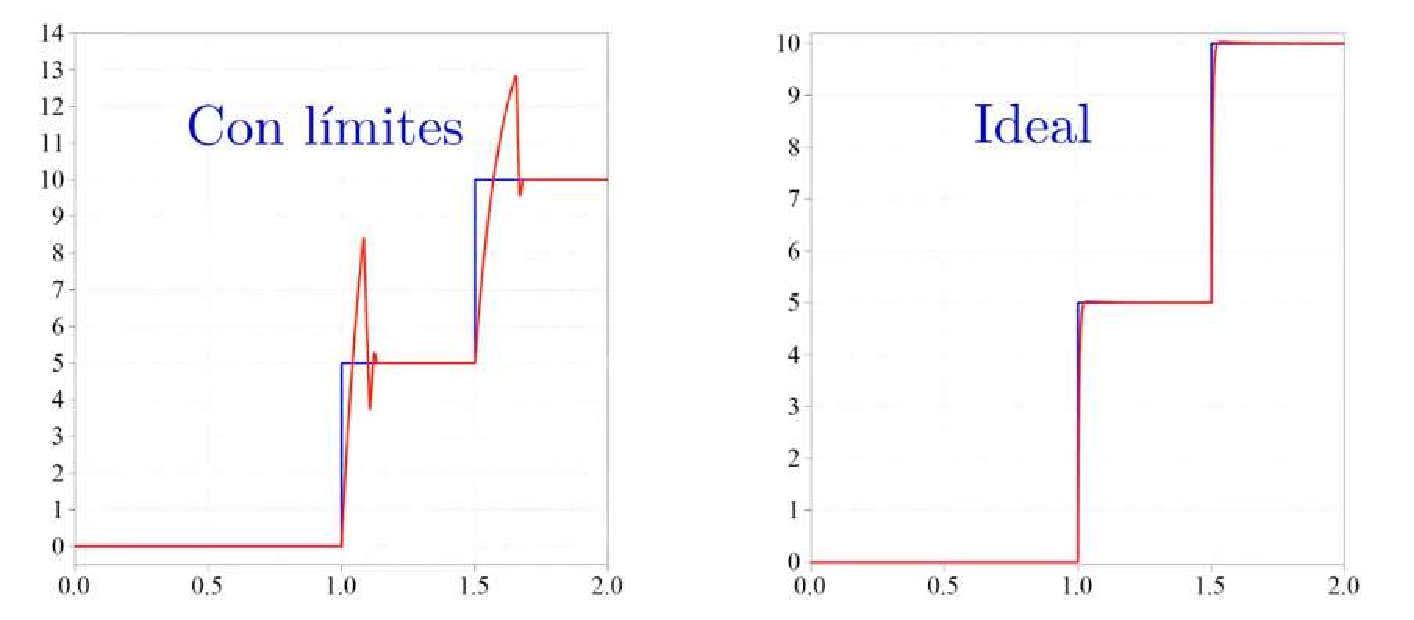
\includegraphics[width=0.4\textwidth]{Auxiliar_6_4} \\
            \textit{Curvas para la obtención de la reactancia saturada y no saturada.}
        \end{center}
        Ademas de la relacion lineal entre la corriente de excitación y corriente de armadura para cortocircuito dado por:
        \begin{center}
            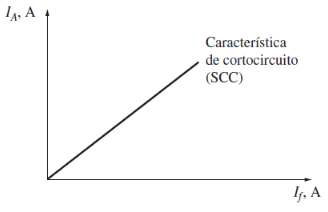
\includegraphics[width=0.44\textwidth]{Auxiliar_6_5} \\
            \textit{Relacion lineal entre la corriente de excitación y corriente de armadura.}
        \end{center}
        Teniendo en cuenta lo anterior, se procede a calcular la reactancia saturada y no saturada de la máquina.
        \subsection*{Reactancia saturada}
        El enunciado entrega la tensión nominal de la máquina en voltaje fase-fase, por lo que se debe transformar un voltaje fase-neutro para que coincidan con los resultados de las pruebas.(\textit{Se debe recordar como se realizan estas pruebas})
        
        \[
        V_{\text{nom}} = \frac{23.9[kVff]}{\sqrt{3}} = 13.7986 \sim 13.8 \, [kV]
        \]
        
        Con lo anterior determinado, se desea obtener la corriente de campo \( I_c \) necesaria para generar una tensión interna nominal \( E = 13.8[kV] \) en los terminales del generador. Para ello, en primer lugar se calcula la pendiente de la curva \( E_a - I_c \) a partir de los datos de la prueba de vacío, eligiendo valores cercanos al punto de tensión deseado.
        \begin{align}
        m &= \frac{14395 - 13100}{240 - 200} = 32.3750
        \end{align}
        A partir de esta pendiente, se obtiene la corriente de campo \( I_c \), con la cual se obtiene una tensión interna nominal.
        \begin{align}
        I_c &= \frac{13800 - 14395}{I_{c}-240} = 221.6216 \, [A]
        \end{align}
        Luego, se desea obtener la corriente de armadura \( I_a \) que se genera cuando existe una corriente de campo \( I_c = 221.6216 [A] \). Para ello, primero se calcula la pendiente de la curva \( I_a - I_c \) a partir de los datos de la prueba de cortocircuito.
        
        \begin{align}
        m_2 &= \frac{2090 - 0}{242 - 0} = 8.6363
        \end{align}
        
        Y por último, se calcula la corriente \( I_a \) a partir de la pendiente.
        
        \begin{align}
        I_a &= \frac{I_{a}- 2090}{221,6216 - 242} = 1914.006 \, [A]
        \end{align}
        
        Finalmente, a partir de estos resultados, se calcula la impedancia saturada del generador.
        
        \begin{align}
        Z_{\text{sat}} &= \frac{E_{\text{nom}}(I_c)}{I_a(I_c)} = \frac{13800[V]}{1913.006[A]} = 7.21[\Omega] \approx x_s
        \end{align}
        
        \subsection*{Reactancia no saturada}
        
        Como no se está considerando la saturación de la curva \( E_a - I_c \), se puede asumir que esta será lineal en todo su recorrido, por lo que se elegirá un punto inicial de dicha curva para calcular la impedancia no saturada.
        
        En particular, para esta ocasión se utilizó un voltaje interno de 5520[V], por lo que se procede a calcular la corriente de armadura \( I_a' \), que se obtiene cuando existe una corriente de campo \( I_c = 61[A] \), a partir de la pendiente de la curva \( I_a - I_c \) calculada anteriormente.
        
        \begin{align}
        \frac{I_{a'}-2090}{61 - 242} = 8.6363 \, [A]\\
        I_{a'} = 526.8297 \, [A]
        \end{align}
        
        Finalmente, a partir de estos resultados, se calcula la impedancia no saturada del generador.
        
        \begin{align}
        Z_{\text{no sat}} &= \frac{E}{I_a'} = \frac{5520}{526.8297} = 10.4778 \, [\Omega]
        \end{align}
        \subsection*{Resolucion 1.2}
       Se debe caracterizar la potencia de la carga con la que se está operando. Para ello, con el factor de potencia entregado (\( fp = 0.85 \) inductivo), se puede obtener el ángulo de la potencia:
    \begin{align}
        \phi &= \arccos(fp) = \arccos(0.85) = 31.79^\circ
    \end{align}
    Mientras que con el dato de la potencia reactiva (\( Q_{3\phi} = 2.5 [MVAr] \)), se puede obtener el módulo de la potencia:
    \begin{align}
        Q_{3\phi} &= |\hat{S}_{3\phi}| \cdot \sin(\phi) \\
        2.5 &= |\hat{S}_{3\phi}| \cdot \sin(0.85) \\
    |\hat{S}_{3\phi}| &= \frac{2.5}{\sin(0.85)} \\
    |\hat{S}_{3\phi}| &= 4.746 \, [MVA]
    \end{align}

Con esto, la potencia aparente será:

\begin{align}
\hat{S}_{3\phi} &= |\hat{S}_{3\phi}| \angle \phi \\
\hat{S}_{3\phi} &= 4.746 \angle 31.79^\circ [MVA]
\end{align}

Y la potencia activa será:

\begin{align}
P_{3\phi} &= |\hat{S}_{3\phi}| \cdot \cos(\phi) \\
P_{3\phi} &= 4.746 \cdot 0.85 \\
P_{3\phi} &= 4.0341 \, [MW]
\end{align}

Luego, las potencias monofásicas serán:

\begin{align}
S_{1\phi} &= \frac{S_{3\phi}}{3} = 1.582 \angle 31.79^\circ \, [MVA] \\
P_{1\phi} &= \frac{P_{3\phi}}{3} = 1.3447 \, [MW] \\
Q_{1\phi} &= \frac{Q_{3\phi}}{3} = 0.8333 \, [MVAr]
\end{align}

Con esto, se puede despejar el fasor de la corriente, imponiendo \( \hat{V} = 13.8 \angle 0^\circ [kV] \) como tensión de referencia:

\begin{align}
\hat{S}_{1\phi} &= \hat{V} \cdot \hat{I}^* \\
I &= \left( \frac{\hat{S}_{1\phi}}{\hat{V}} \right)^* \\
I &= \left( \frac{1.582 \angle 31.79^\circ \, [MW]}{13.8 \angle 0^\circ \, [kV]} \right)^* \\
I &= 114.6362 \angle -31.79^\circ \, [A]
\end{align}

(\textit{No olvidar adicionar el conjugado, dado que este valor produce un cambio de fase, equivalentemente a adicionar un signo - en la exponencial}) Finalmente, para obtener los valores de \(E\) y \(\delta\), se consideran las siguientes ecuaciones:

\begin{align}
P_{1\phi} &= \frac{V \cdot E}{x_s} \sin(\delta) \\
Q_{1\phi} &= \frac{V}{x_s} \left( E \cdot \cos(\delta) - V \right)
\end{align}

Elevando al cudrado ambas expresiones y sumando se obtiene tiene:

\begin{align}
\frac{P_{1\phi} \cdot x_s}{V} &= E \cdot \sin(\delta) \\
\frac{Q_{1\phi} \cdot x_s}{V} + V &= E \cdot \cos(\delta)
\end{align}

Sumando las dos expresiones anteriores se tiene:

\begin{align}
E^2 \cdot \left( \cos^2(\delta) + \sin^2(\delta) \right) &= \left( \frac{P_{1\phi} \cdot x_s}{V} \right)^2 + \left( \frac{Q_{1\phi} \cdot x_s}{V} + V \right)^2
\end{align}

Por lo que:

\begin{align}
E &= \sqrt{\left( \frac{P_{1\phi} \cdot x_s}{V} \right)^2 + \left( \frac{Q_{1\phi} \cdot x_s}{V} + V \right)^2}
\end{align}
Esta expresion recomiendo recodarla, dado que es general y siempre es posible utilizarla y permite obtener E sin que dependa explicitamente de \( \delta \). Finalmente:
\begin{align}
|E| &= 14.2527 \, [kV]
\end{align}
Luego se puede reemplazar este E en calcular de las expresiones anteriores con tal de obtener el valor de \( \delta \), resultando en:
\begin{align}
\delta &= 2.83^\circ \\
\hat{E} &= 14.2527 \angle 2.83^\circ [kV]
\end{align}
\subsection*{Resolucion 1.3}
Una vez obtenido lo anterior, es posible el graficar el diagrama fasorial para saber como se encuentra operando el generador, es util recordar las diferentes formas de operaciones las cuales vienen dadas en:
\begin{center}
    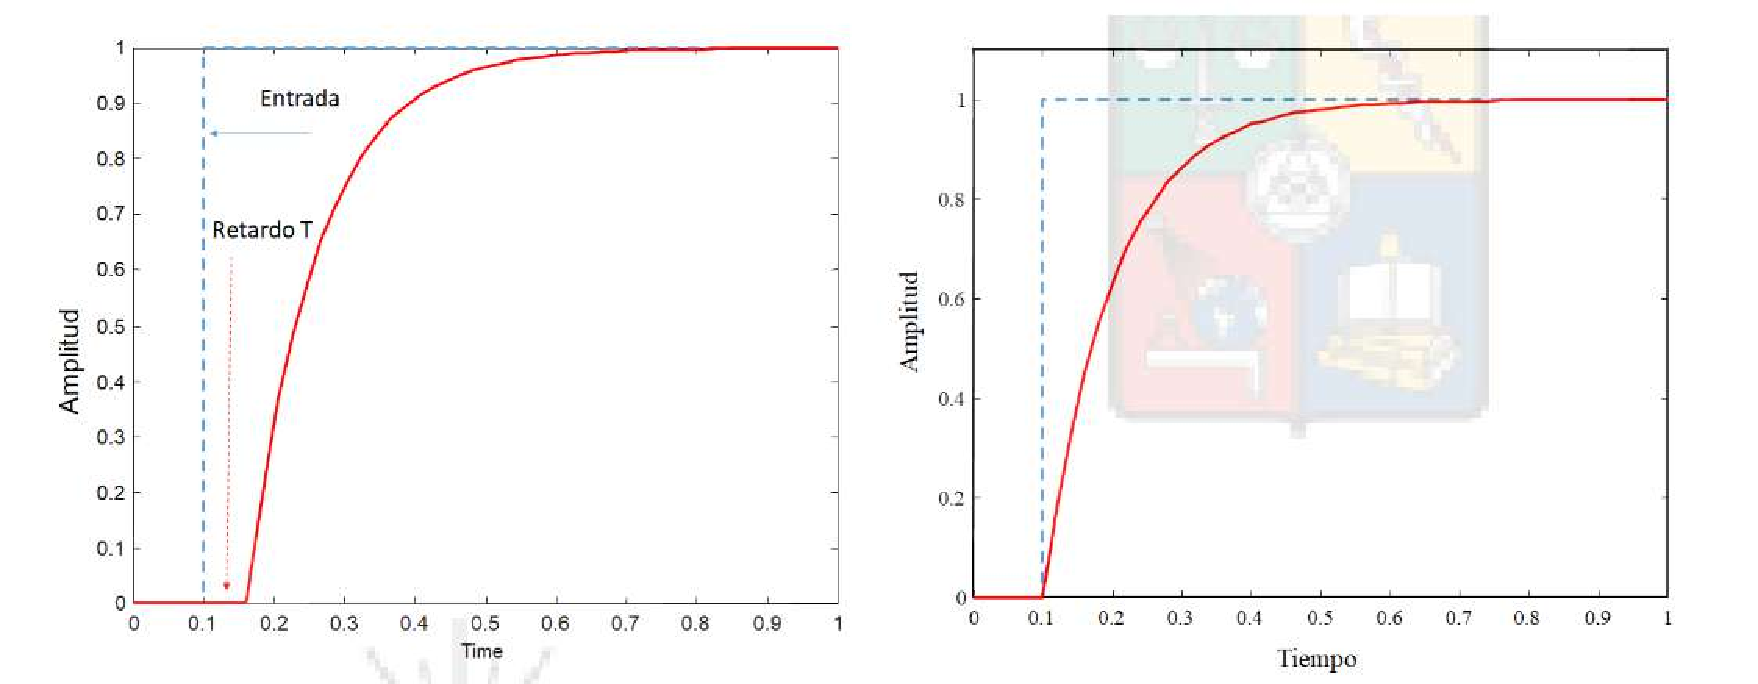
\includegraphics[width=0.7\textwidth]{Auxiliar_6_6} \\
    \textit{Diagramas fasoriales para las diferentes formas de operación, tanto para generador como motor.}
\end{center}
Luego se tiene que para nuestro caso particular\\\\
\begin{center}
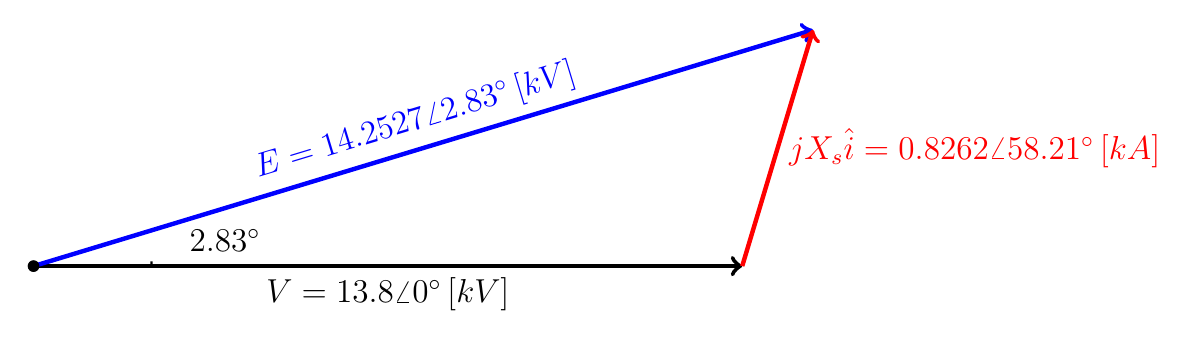
\begin{tikzpicture}

    % Definir los puntos
    \coordinate (O) at (0,0); % Origen
    \coordinate (V) at (9,0); % Punto V
    \coordinate (E) at (9.9,3); % Punto E con el ángulo
    
    % Dibujar las líneas más gruesas
    \draw[->, ultra thick, black] (O) -- (V) node[midway, below] {\large $V = 13.8 \angle 0^\circ \, \text{[kV]}$}; % Línea V
    \draw[->, ultra thick, blue] (O) -- (E) node[midway, above, sloped] {\large $E = 14.2527 \angle 2.83^\circ \, \text{[kV]}$}; % Línea E
    \draw[->, ultra thick, red] (V) -- (E) node[midway, right] {\large $jX_{s}\hat{i} = 0.8262 \angle 58.21^\circ \, \text{[kA]}$}; % Línea corriente
    
    % Dibujar el ángulo con mejor ubicación
    \draw[thick] (1.5,0) arc[start angle=0,end angle=2.83,radius=1.2] node[above right, xshift=10] {\large $2.83^\circ$};
    
    % Añadir un punto para hacer el ángulo más visible
    \node at (O) [circle,fill,inner sep=1.5pt] {};
    
    \end{tikzpicture}
\end{center}
    \vspace{0.5cm}
    
    Como $E > V$ se concluye que el generador está sobreexcitado, por lo que la máquina está inyectando potencia reactiva al sistema.
    \subsection*{Resolucion 1.4}

    La velocidad de giro se calcula a partir de los datos de la \textit{frecuencia de la red} y de la \textit{cantidad de polos} con la siguiente fórmula:

\begin{align}
n_s &= \frac{120 \cdot f}{p} = \frac{120 \cdot 50 \, [Hz]}{4} = 1500 \, [rpm]
\end{align}

\[
\Rightarrow \omega_s = \frac{2 \pi n_s}{60} = 157.0796 \, [rad/s]
\]

Con esto, el torque será:

\begin{align}
\tau &= \frac{P_{3\phi}}{\omega_s} = \frac{\text{Re}\{ 3 \cdot E \cdot I^* \}}{\omega_s} \approx \frac{\text{Re}\{ 3 \cdot V \cdot I^* \}}{\omega_s} \\
\tau &= \frac{4.0341 \, [MW]}{157.0796 \, [rad/s]} \\
\tau &= 25.6818 \, [kNm]
\end{align}
Luego se busca obtener la variable de control que  permite llevar al generador a operar con factor de potencia unitario manteniendo el módulo de la tensión interna \(E\)

Es decir que se desea pasar de \(fp_1 = 0.85\) inductivo a \(fp_2 = 1\), lo que quiere decir que:

\[
\phi_2 = \arccos(fp_2) = \arccos(1) = 0^\circ
\]

\[
\Rightarrow Q_{3\phi} = S_{3\phi} \cdot \sin(0^\circ) = 0
\]

Por otro lado, las variables controlables de una máquina síncrona son el \textit{torque} \(\tau\) generado por las turbinas (el cual modificará la potencia activa \(P\), y por consiguiente, el ángulo \(\delta\)) y la \textit{corriente de campo} \(I_c\) (la cual afectará directamente la tensión interna \(E\)). Luego, como se desea mantener el módulo de \(E\), la única variable a modificar será el torque.

Con esto en mente, primero se calcula cuánto se modifica el ángulo \(\delta\):

\begin{align}
Q_{3\phi} &= 0 = 3 \cdot \frac{V}{x_s} \left( E \cdot \cos(\delta) - V \right) \\
0 &= 3 \cdot \frac{V}{x_s} \left( E \cdot \cos(\delta) - V \right) \\
\Rightarrow E \cdot \cos(\delta) &= V
\end{align}

\[
\Rightarrow \delta = \arccos \left( \frac{V}{E} \right)
\]

\[
\delta = \arccos \left( \frac{13800}{14252.7} \right)
\]

\[
\delta = 14.48^\circ
\]

Con este nuevo ángulo se calcula la nueva potencia activa:

\begin{align}
P_{3\phi} &= 3 \cdot \frac{V \cdot E}{x_s} \cdot \sin(\delta) \\
P_{3\phi} &= 3 \cdot \frac{13800 \cdot 14252.7}{7.21} \cdot \sin(14.48^\circ) \\
P_{3\phi} &= 20.4633 \, [MW]
\end{align}

Y finalmente se calcula el torque:

\begin{align}
\tau &= \frac{P_{3\phi}}{\omega_s} \\
\tau &= \frac{20.4633 \, [MW]}{157.0796 \, [rad/s]} \\
\tau &= 130.2734 \, [kNm]
\end{align}

Finalmente para determinar la regulación de tensión en el nuevo punto de operación encontrado en la parte c):

\[
\text{Reg} = \frac{E - V_{\text{fuente}}}{V_{\text{fuente}}} = \frac{14252.7 \, [kV] - 13800 \, [kV]}{13800 \, [kV]} = 0.0328
\]
    \end{solution}
    %%%%%%%%%%%%%%%%%%%%%%%%%%%
    \question Se tiene un generador síncrono trifásico de potencia nominal 60 $[\text{MVA}]$ y tensión nominal 23 $[\text{kV}]$ que se encuentra conectado a una barra infinita de igual tensión nominal y frecuencia 50 $[\text{Hz}]$. La máquina posee una reactancia de 5 $[\Omega]$ por fase y cuenta con 24 polos.

    En cierto instante, la máquina inyecta a la red una corriente de 1.2 $[\text{kA}]$ por fase, con factor de potencia 0.87 inductivo.
    
    A partir de esto, calcular:
    
    \begin{enumerate}
        \item[a)] La potencia activa, reactiva y aparente en los terminales de la máquina.
        \item[b)] La tensión interna y el ángulo de carga. Dibujar el diagrama fasorial.
        \item[c)] La velocidad a la que gira la máquina y el torque que esta ejerce.
        \item[d)] En cierto instante, el operador cambia el factor de potencia de la máquina a 0.9 capacitivo manteniendo la potencia activa suministrada a la red. Determine nuevamente la tensión interna y el ángulo de carga de la máquina y dibuje el respectivo diagrama fasorial.
    \end{enumerate}
%%%%%%%%%%%%%%%%%%%%%%%%%%%
\begin{solution}
\subsection*{Resolucion 2.1}
En primer lugar, definimos los valores de los \textit{corriente} y \textit{voltaje} en los terminales.
\[
V_{fn} = \frac{23[kV_{ff}]}{\sqrt{3}} = 13.2791 \, [kV]
\]
En donde imponemos que el voltaje en los terminales será nuestra referencia.
\[
\Rightarrow \hat{V} = 13.2791 \angle 0^\circ \, [kV]
\]
Luego, como tenemos el valor del módulo de la corriente pero no del ángulo, lo dejamos expresado de la siguiente forma:
\[
\hat{I} = 1.2 \angle \delta_{I} \, [kA]
\]
Por otro lado, a partir del dato del factor de potencia se puede calcular el ángulo de la potencia:
\begin{align}
\phi &= \arccos(fp) = \arccos(0.87) = 29.54^\circ
\end{align}
A partir de lo anterior, podemos calcular la potencia a partir de la siguiente expresión:
\begin{align}
\hat{S}_{3\phi} &= 3 \cdot \hat{V} \cdot \hat{I}^*
\end{align}
En donde primero se obtiene el módulo de la potencia:
\begin{align}
|\hat{S}_{3\phi}| &= 3 \cdot |\hat{V}| \cdot |\hat{I}| \\
|\hat{S}_{3\phi}| &= 3 \cdot 13.2791 \, [kV] \cdot 1.2 \, [kA] \\
|\hat{S}_{3\phi}| &= 47.8048 \, [MVA]
\end{align}
Y como ya se tiene el ángulo de la potencia, se procede a despejar el ángulo de la corriente:
\begin{align}
\angle \hat{S}_{3\phi} &= \angle \hat{V} + (- \angle \hat{I}) \\
29.54^\circ &= 0^\circ - \delta_{I} \\
\Rightarrow \delta_{I} &= -29.54^\circ
\end{align}
Finalmente, los valores de la corriente y la potencia aparente serán los que se muestran a continuación:
\begin{align}
\hat{I} &= 1.2 \angle -29.54^\circ \, [kA] \\
\hat{S}_{3\phi} &= 47.8048 \angle 29.54^\circ \, [MVA]
\end{align}
Y a partir de esto se puede calcular la potencia activa y reactiva:
\begin{align}
P_{3\phi} &= |\hat{S}_{3\phi}| \cdot \cos(\phi) = 47.8048 \cdot \cos(29.54^\circ) = 41.5907 \, [MW] \\
Q_{3\phi} &= |\hat{S}_{3\phi}| \cdot \sin(\phi) = 47.8048 \cdot \sin(29.54^\circ) = 23.5693 \, [MVAr]
\end{align}
\subsection*{Resolucion 2.2}
Al igual que antes se busca realizar el diagrama fasorial por lo que se obtiene $\hat{E}$ tal que:
\begin{align}
    \hat{E} &= j \cdot x_s \cdot \hat{I} + \hat{V} \\
    \hat{E} &= j \cdot 5[\Omega] \cdot (1.2 \angle -29.54^\circ \, [kA]) + 13.2791 \angle 0^\circ \, [kV] \\
    \hat{E} &= 17.0557 \angle 17.82^\circ \, [kV]
    \end{align}
    \begin{center}
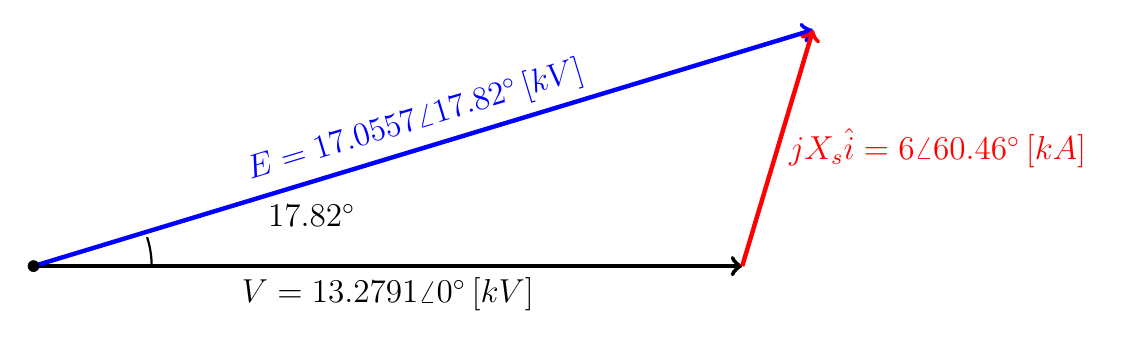
\begin{tikzpicture}

    % Definir los puntos
    \coordinate (O) at (0,0); % Origen
    \coordinate (V) at (9,0); % Punto V
    \coordinate (E) at (9.9,3); % Punto E con el ángulo
    
    % Dibujar las líneas más gruesas
    \draw[->, ultra thick, black] (O) -- (V) node[midway, below] {\large $V = 13.2791 \angle 0^\circ \, \text{[kV]}$}; % Línea V
    \draw[->, ultra thick, blue] (O) -- (E) node[midway, above, sloped] {\large $E = 17.0557 \angle 17.82^\circ \, \text{[kV]}$}; % Línea E
    \draw[->, ultra thick, red] (V) -- (E) node[midway, right] {\large $jX_{s}\hat{i} = 6 \angle 60.46^\circ \, \text{[kA]}$}; % Línea corriente
    
    % Dibujar el ángulo con mejor ubicación
    \draw[thick] (1.5,0) arc[start angle=0,end angle=17.82,radius=1.2] node[above right, xshift=40 ] {\large $17.82^\circ$};
    
    % Añadir un punto para hacer el ángulo más visible
    \node at (O) [circle,fill,inner sep=1.5pt] {};
    
    \end{tikzpicture}
\end{center}
    Como $E > V$ se tendrá un generador sobreexitado, por lo que la máquina está inyectando potencia reactiva al sistema.
    \subsection*{Resolucion 2.3}
    La velocidad de giro de la máquina se obtiene a partir de la frecuencia de la red y de la cantidad de polos con la siguiente fórmula:

\begin{align}
n_s &= \frac{120 \cdot f}{p} = \frac{120 \cdot 50 \, [Hz]}{24} = 250 \, [rpm]
\end{align}

\[
\Rightarrow \omega_s = \frac{2\pi \cdot n_s}{60} = 26.1799 \, [rad/s]
\]

Con esto, el torque será:

\begin{align}
\tau &= \frac{P_{3\phi}}{\omega_s} \\
\tau &= \frac{3 \cdot \text{Re} \left\{ \hat{E} \cdot \hat{V}^* \right\}}{\omega_s} \\
\tau &= \frac{41.5907 \, [MW]}{26.1799 \, [rad/s]} \\
\tau &= 1.5887 \, [MNm]
\end{align}
\subsection*{Resolucion 2.4}
Se pasa de \( fp = 0.87 \) inductivo a \( fp' = 0.9 \) capacitivo. Este cambio significará una modificación en el ángulo \(\phi\) con un signo -:

\begin{align}
\phi &= - \arccos(fp') = - \arccos(0.9) = -25.84^\circ
\end{align}

Por otro lado, se desea mantener la potencia activa con la que se estaba operando, por lo que la potencia aparente se verá modificada de la siguiente manera:

\begin{align}
P_{3\phi} &= |\hat{S}_{3\phi}| \cdot \cos(\phi) \\
\Rightarrow |\hat{S}_{3\phi}| &= \frac{P_{3\phi}}{\cos(\phi)} \\
|\hat{S}_{3\phi}| &= \frac{41.5907 \, [MW]}{0.9} \\
|\hat{S}_{3\phi}| &= 46.2112 \, [MVA]
\end{align}

Con lo anterior, la expresión para la potencia aparente nueva será:

\[
\hat{S}_{3\phi} = 46.2112 \angle -25.84^\circ \, [MVA]
\]

Además, como se tiene una nueva potencia aparente, entonces se tendrá una nueva corriente.

\[
\hat{S}_{1\phi} = \hat{V} \cdot \hat{I}^*
\]

\begin{align}
\hat{I}^* &= \left( \frac{\hat{S}_{1\phi}}{\hat{V}} \right)^* \\
\hat{I} &= \left( \frac{46.2112 \angle -25.84^\circ \, [MVA]}{3 \cdot 13.2791 \angle 0^\circ \, [kV]} \right)^* \\
\hat{I} &= (1.16 \angle -25.84^\circ) \, [kA] \\
\hat{I} &= 1.16 \angle 25.84^\circ \, [kA]
\end{align}

Finalmente, la tensión interna de la máquina se calculará de la siguiente manera:

\begin{align}
\hat{E} &= j \cdot x_s \cdot \hat{I} + \hat{V} \\
\hat{E} &= j \cdot 5[\Omega] \cdot (1.16 \angle 25.84^\circ \, [kA]) + 13.2791 \angle 0^\circ \, [kV] \\
\hat{E} &= 11.9514 \angle 25.90^\circ \, [kV]
\end{align}

\begin{center}
    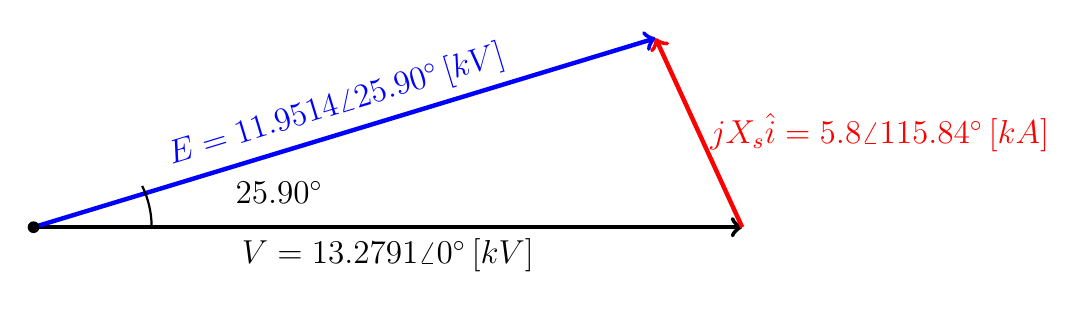
\begin{tikzpicture}
    
    % Definir los puntos
    \coordinate (O) at (0,0); % Origen
    \coordinate (V) at (9,0); % Punto V
    \coordinate (E) at (7.9,2.4); % Punto E con el ángulo
    
    % Dibujar las líneas más gruesas
    \draw[->, ultra thick, black] (O) -- (V) node[midway, below] {\large $V = 13.2791 \angle 0^\circ \, \text{[kV]}$}; % Línea V
    \draw[->, ultra thick, blue] (O) -- (E) node[midway, above, sloped] {\large $E = 11.9514 \angle 25.90^\circ \, \text{[kV]}$}; % Línea E
    \draw[->, ultra thick, red] (V) -- (E) node[midway, right] {\large $jX_{s}\hat{i} = 5.8 \angle 115.84^\circ \, \text{[kA]}$}; % Línea corriente
    
    % Dibujar el ángulo con mejor ubicación
    \draw[thick] (1.5,0) arc[start angle=0,end angle=25.90,radius=1.2] node[above right, xshift=30, yshift=-10] {\large $25.90^\circ$};
    
    % Añadir un punto para hacer el ángulo más visible
    \node at (O) [circle,fill,inner sep=1.5pt] {};
    
    \end{tikzpicture}
    \end{center}
    
Notar que al cambiar el factor de potencia de 0.87 inductivo a uno de 0.9 capacitivo significó pasar de operar un generador sobreexcitado a uno subexcitado, lo que se traduce en que pasamos de inyectar reactivos de la red a consumirlos.

Para cuantificar esta variación utilizamos la siguiente ecuación que relaciona la tensión interna con la corriente de campo:

\[
E = K \cdot \omega \cdot I_c
\]

\[
\Rightarrow I_c = \frac{E}{K \cdot \omega}
\]

Con esto, la variación de la corriente de campo para cambiar entre los puntos de operación fue de:

\begin{align}
\Delta I_c &= \frac{I_{c1} - I_{c0}}{I_{c0}} \\
\Delta I_c &= \frac{\frac{E_1}{K \cdot \omega} - \frac{E_0}{K \cdot \omega}}{\frac{E_0}{K \cdot \omega}} \\
\Delta I_c &= \frac{E_1 - E_0}{E_0} \\
\Delta I_c &= \frac{11.9514 \, [kV] - 17.0557 \, [kV]}{17.0557 \, [kV]} \\
\Delta I_c &= -0.2993 = -29.93 \%
\end{align}

 \end{solution}
%%%%%%%%%%%%%%%%%%%%%%%%%%%
\question Una máquina síncrona trifásica (máquina de CA) se conecta mecánicamente a una máquina de CC en derivación y forman un conjunto de motor-generador como el que se muestra en la Figura 4. La máquina de CC se conecta a un sistema de potencia de CC que suministra 240 [V] constantes y la máquina de CA se conecta a una barra infinita de 480 [V] y 60 [Hz]. La máquina de CC tiene cuatro polos y sus valores nominales son: 50 [kW] y 240 [V]. Tiene una resistencia del inducido por unidad de 0.03456 [$\Omega$]. La máquina de CA tiene cuatro polos y está conectada en estrella. Sus valores nominales son de 50 [kVA], 480 [V], un factor de potencia de 0.8 en retraso y su reactancia síncrona saturada es de 3.0 [$\Omega$] por fase. Se pueden despreciar todas las pérdidas excepto las de resistencia del inducido de la máquina de CC. Suponga que las curvas de magnetización de ambas máquinas son lineales.

\begin{figure}[h!]
    \centering
    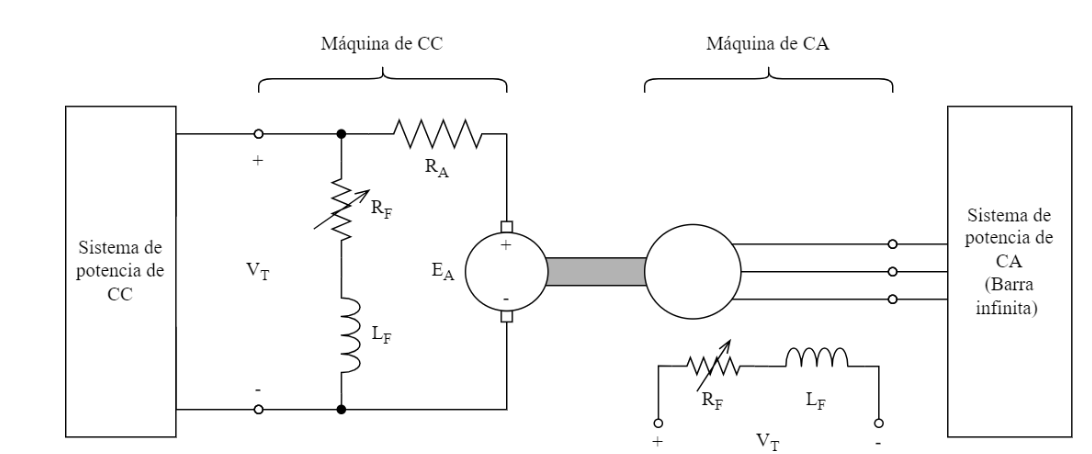
\includegraphics[width=0.7\textwidth]{Auxiliar_6_1}
    \caption{Conjunto Motor-Generador.}
\end{figure}

Inicialmente, la máquina de CA suministra 50 [kVA] con un factor de potencia de 0.8 en retraso al sistema de potencia de CA.
\begin{enumerate}
    \item ¿Cuánta potencia se suministra al motor de CC desde el sistema de potencia de CC?
    \item ¿De qué magnitud es la tensión interna generada $E_A$ de la máquina de CC?
    \item ¿Cuál es la magnitud y el ángulo de la tensión interna generada E de la máquina de
    CA?
    \item Bosqueje un diagrama fasorial de la máquina sincrónica en el punto de operación anterior
\end{enumerate}
%%%%%%%%%%%%%%%%%%%%%%%%%%%
\begin{solution}
   \subsection*{Resolucion 3.1}
   Es posible analizar el problema pensando en que cada uno de los elementos de el conjunto motor-generador era una caja con potencias de entrada y salida de la siguiente manera, tal que:
   \begin{center}
    \begin{tikzpicture}[auto, node distance=2cm,>=latex']
    
    % Definir los nodos
    \node[circle, draw, align=center] (redcc) {RED\\ CC};
    \node[rectangle, draw, right of=redcc, node distance=3cm] (cc) {CC};
    \node[rectangle, draw, right of=cc, node distance=4cm] (ca) {CA};
    \node[circle, draw, right of=ca, node distance=3cm, align=center] (redca) {RED\\ CA};
    
    % Dibujar las flechas
    \draw[->] (redcc) -- node {$P_{cc\_in}$} (cc);
    \draw[->] (cc) -- node {$P_{cc\_out} = P_{ca\_in}$} (ca);
    \draw[->] (ca) -- node {$P_{ca\_out}$} (redca);
    
    \end{tikzpicture}
    \end{center}
    Ahora, como se poseen los datos asociados a la red de corriente alterna, lo que se debe hacer es analizar las potencias de entrada y salida de cada bloque partiendo por la red alterna hacia la red de corriente continua y así obtener la potencia que entra a la máquina de corriente continua \( P_{cc\_in} \).
    
    Partiendo por la red de corriente alterna, se sabe que la máquina suministra una potencia aparente de 50 kVA en retraso, por lo tanto es de carácter inductivo y el signo asociado al factor de potencia es positivo por lo que basta con usar el valor de 0.8 de la siguiente manera:
    
    \begin{align}
    P_{ca\_out} &= 50 \cdot \cos(\theta) \\
    P_{ca\_out} &= 50 \cdot 0.8 \\
    P_{ca\_out} &= 40 \, [kW]
    \end{align}
    
    El enunciado menciona que se pueden despreciar todas las pérdidas de la máquina de corriente continua por lo que se tiene que:
    
    \begin{align}
    P_{ca\_in} &= P_{ca\_out} = 40 \, [kW]
    \end{align}
    
    Luego, asumiendo que no hay pérdidas en el eje que conecta la máquina de corriente continua con la máquina de corriente alterna:
    
    \begin{align}
    P_{ca\_in} &= P_{cc\_out}
    \end{align}
    
    La potencia de salida de la máquina de corriente continua corresponde a la potencia eléctrica de esta:
    
    \begin{align}
    P_{cc\_out} &= P_{electrica} = E_a \cdot i_a = 40 \, [kW]
    \end{align}
    
    Teniendo en cuenta que si se tienen pérdidas en la resistencia del inducido de la máquina CC se tiene que la potencia de entrada se relaciona con la de salida de la siguiente manera:
    
    \begin{align}
    P_{cc\_in} &= P_{cu} + P_{cc\_out}
    \end{align}
    
    Donde:
    
    \begin{align}
    P_{cu} &= i_a^2 \cdot R_a
    \end{align}
    
    Donde la corriente \( i_a \) es desconocida por lo que se utiliza la siguiente ecuación de la máquina de corriente continua operando como motor para obtenerla:
    
    \begin{align}
    E_a &= V_r - R_a \cdot i_a \\
    E_a &= 240 - 0.03456 \cdot i_a
    \end{align}
    
    Reemplazando en la ecuación de la potencia eléctrica se obtiene la relación que permite obtener la corriente:
    
    \begin{align}
    P_{electrica} &= 40 \, [kW] = (240 - 0.03456 \cdot i_a) \cdot i_a
    \end{align}
    
    \begin{align}
    0.03456 \cdot i_a^2 - 240 \cdot i_a + 40000 &= 0
    \end{align}
    
    Donde se obtienen los siguientes resultados:
    
    \begin{align}
    i_{a1} &= 6773.57 \, [A] \\
    i_{a2} &= 170.87 \, [A]
    \end{align}
    
    Donde se escoge \( i_a = 170.87 \, [A] \) ya que el primer valor es muy grande, más cercano a una corriente obtenida en un cortocircuito.
    
    Finalmente, volviendo a las pérdidas en la resistencia \( R_a \) y reemplazando el valor de la corriente:
    
    \begin{align}
    P_{cu} &= (170.87)^2 \cdot 0.03456 \\
    P_{cu} &= 1009.0448 \, [W] = 1.009 \, [kW]
    \end{align}
    
    Por lo tanto, la potencia que se suministra al motor CC es de:
    
    \begin{align}
    P_{cc\_in} &= 40 \, [kW] + 1.009 \, [kW] = 41.009 \, [kW]
    \end{align}
    \subsection*{Resolucion 3.2}
    La magnitud de la tensión interna \( E_a \) está dada por la corriente obtenida en la parte anterior.

\begin{align}
E_a &= V_T - R_a \cdot i_a \\
E_a &= 240 - 0.03456 \cdot 170.871 \\
E_a &= 234.0946 \, [V]
\end{align}
\subsection*{Resolucion 3.3 }
Como la máquina de corriente alterna está funcionando como generador, su ecuación de tensión interna asociada es la siguiente:

\begin{align}
\hat{E} &= j \cdot X_s \cdot \hat{i} + V
\end{align}

Donde se tiene que:

\begin{align}
V &= \frac{480}{\sqrt{3}} \, [V_{ff}] = 277.1281 \angle 0 \, [V_{fn}]
\end{align}

La potencia trifásica es la siguiente:

\begin{align}
S_{3\phi} &= |S_{3\phi}| \angle \phi = 50 \angle \arccos(0.8) = 50 \angle 36.86^\circ \, [MV A]
\end{align}

Por lo tanto, la corriente es:

\begin{align}
\hat{i} &= \left( \frac{S_{3\phi}}{3 \cdot V} \right)^* = \left( \frac{50 \angle 36.86^\circ \, [MV A]}{3 \cdot 277.1281 \angle 0 \, [V_{fn}]} \right)^* \\
\hat{i} &= 60.1406 \angle -36.86^\circ \, [A]
\end{align}

Por lo tanto, la tensión interna de la máquina es:

\begin{align}
\hat{E} &= j \cdot 3 \cdot 60.1406 \angle -36.86^\circ + 277.1281 \angle 0 \\
\hat{E} &= 411.5071 \angle 20.53^\circ \, [V]
\end{align}
\subsection*{Resolucion 3.4}
Luego dibujamos el diagrama fasorial, tal que:
\begin{center}
    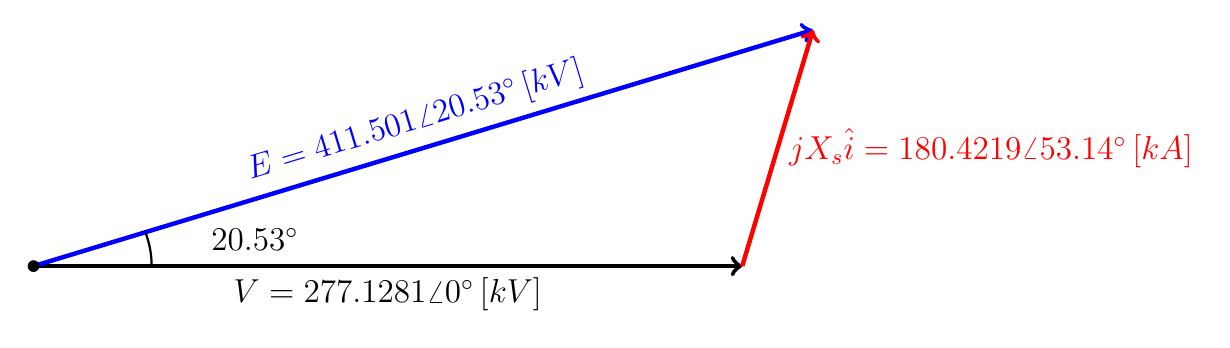
\begin{tikzpicture}
    
        % Definir los puntos
        \coordinate (O) at (0,0); % Origen
        \coordinate (V) at (9,0); % Punto V
        \coordinate (E) at (9.9,3); % Punto E con el ángulo
        
        % Dibujar las líneas más gruesas
        \draw[->, ultra thick, black] (O) -- (V) node[midway, below] {\large $V = 277.1281 \angle 0^\circ \, \text{[kV]}$}; % Línea V
        \draw[->, ultra thick, blue] (O) -- (E) node[midway, above, sloped] {\large $E = 411.501 \angle 20.53^\circ \, \text{[kV]}$}; % Línea E
        \draw[->, ultra thick, red] (V) -- (E) node[midway, right] {\large $jX_{s}\hat{i} = 180.4219 \angle 53.14^\circ \, \text{[kA]}$}; % Línea corriente
        
        % Dibujar el ángulo con mejor ubicación
        \draw[thick] (1.5,0) arc[start angle=0,end angle=20.53,radius=1.2] node[above right, xshift=20, yshift=-10] {\large $20.53^\circ$};
        
        % Añadir un punto para hacer el ángulo más visible
        \node at (O) [circle,fill,inner sep=1.5pt] {};
        
        \end{tikzpicture}
    \end{center}
\end{solution}
%%%%%%%%%%%%%%%%%%%%%%%%%%%

\end{questions}
\newpage
%%%%%%%%%%%%%%%%%%%%%%%%%%%
\section{Resumen}
\begin{itemize}
    \item \textbf{Velocidad síncrona} \\
    La máquina síncrona elemental corresponde a una máquina de voltaje alterno sinusoidal cuya frecuencia eléctrica $\omega$ es igual a la velocidad mecánica $\omega_m$, la cual se denomina velocidad de sincronismo $\omega_s$.
    
    \[
    \omega_s = \frac{2\pi \cdot n_s}{60} = 2\pi f
    \]
    
    De forma general, para una máquina con un enrollado de estator de $p$ polos, se tiene que la frecuencia $\omega$ del voltaje generado está relacionada con la velocidad angular mecánica $\omega_m$ mediante:
    
    \[
    \omega = \frac{p}{2} \cdot \omega_m \quad \Rightarrow \quad n_s = \frac{120 \cdot f}{p}
    \]
    
    \item \textbf{Modelos circuitales} \\
    Motor:
    \begin{center}
        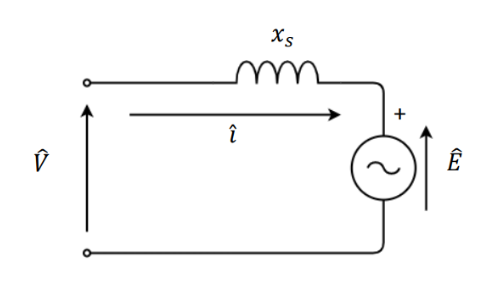
\includegraphics[width=0.5\textwidth]{Auxiliar_6_2.png}
    \end{center}
    
    \[
    \hat{V} = \hat{E} + j \cdot x_s \cdot \hat{i}
    \]
    
    Generador:
    \begin{center}
            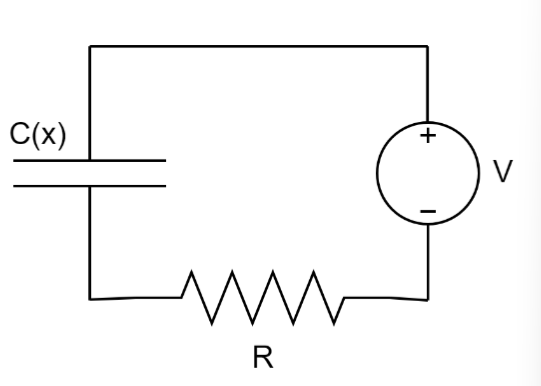
\includegraphics[width=0.5\textwidth]{Auxiliar_6_3.png}
    \end{center}
    
    \[
    \hat{E} = \hat{V} + j \cdot x_s \cdot \hat{i}
    \]
    
    \item \textbf{Potencias} \\
    En estado estacionario, las potencias $P$ y $Q$ se calculan mediante:
    
    \[
    P_{1\Phi} = \frac{V \cdot E}{x_s} \sin(\delta)
    \]
    
    \[
    Q_{1\Phi} = \frac{V}{x_s} \left( E \cdot \cos(\delta) - V \right)
    \]
    
    A partir de lo anterior, la máquina síncrona puede tener distintas formas de operación:
    
    \begin{itemize}
        \item Si $P > 0$ la máquina actúa como generador.
        \item Si $P < 0$ la máquina actúa como motor.
        \item Si $Q > 0$ la máquina se encuentra sobreexcitada.
        \item Si $Q < 0$ la máquina se encuentra subexcitada.
    \end{itemize}
    
    \item \textbf{Torque mecánico} \\
    \[
    T_m = \frac{P_{3\Phi}}{\omega_s}
    \]
    
\end{itemize}

\end{document}